\documentclass[dvipsnames,crop,tikz,border=1px]{standalone}
\usepackage{xcolor}
\usepackage{amsmath}
%\usepackage{lmodern}
%\SetSymbolFont{letters}{bold}{OML}{cmbr}{bx}{it}
\renewcommand{\familydefault}{\sfdefault}

\newcommand{\data}[1]{\quad(\textsc{#1})}
\newcommand{\ellipsis}{\textbf{[\(\boldsymbol\ldots\)]}}
\newcommand{\hl}[1]{\colorbox{red!10}{#1}}

\usetikzlibrary{matrix,arrows,positioning,scopes,shapes}

\begin{document}
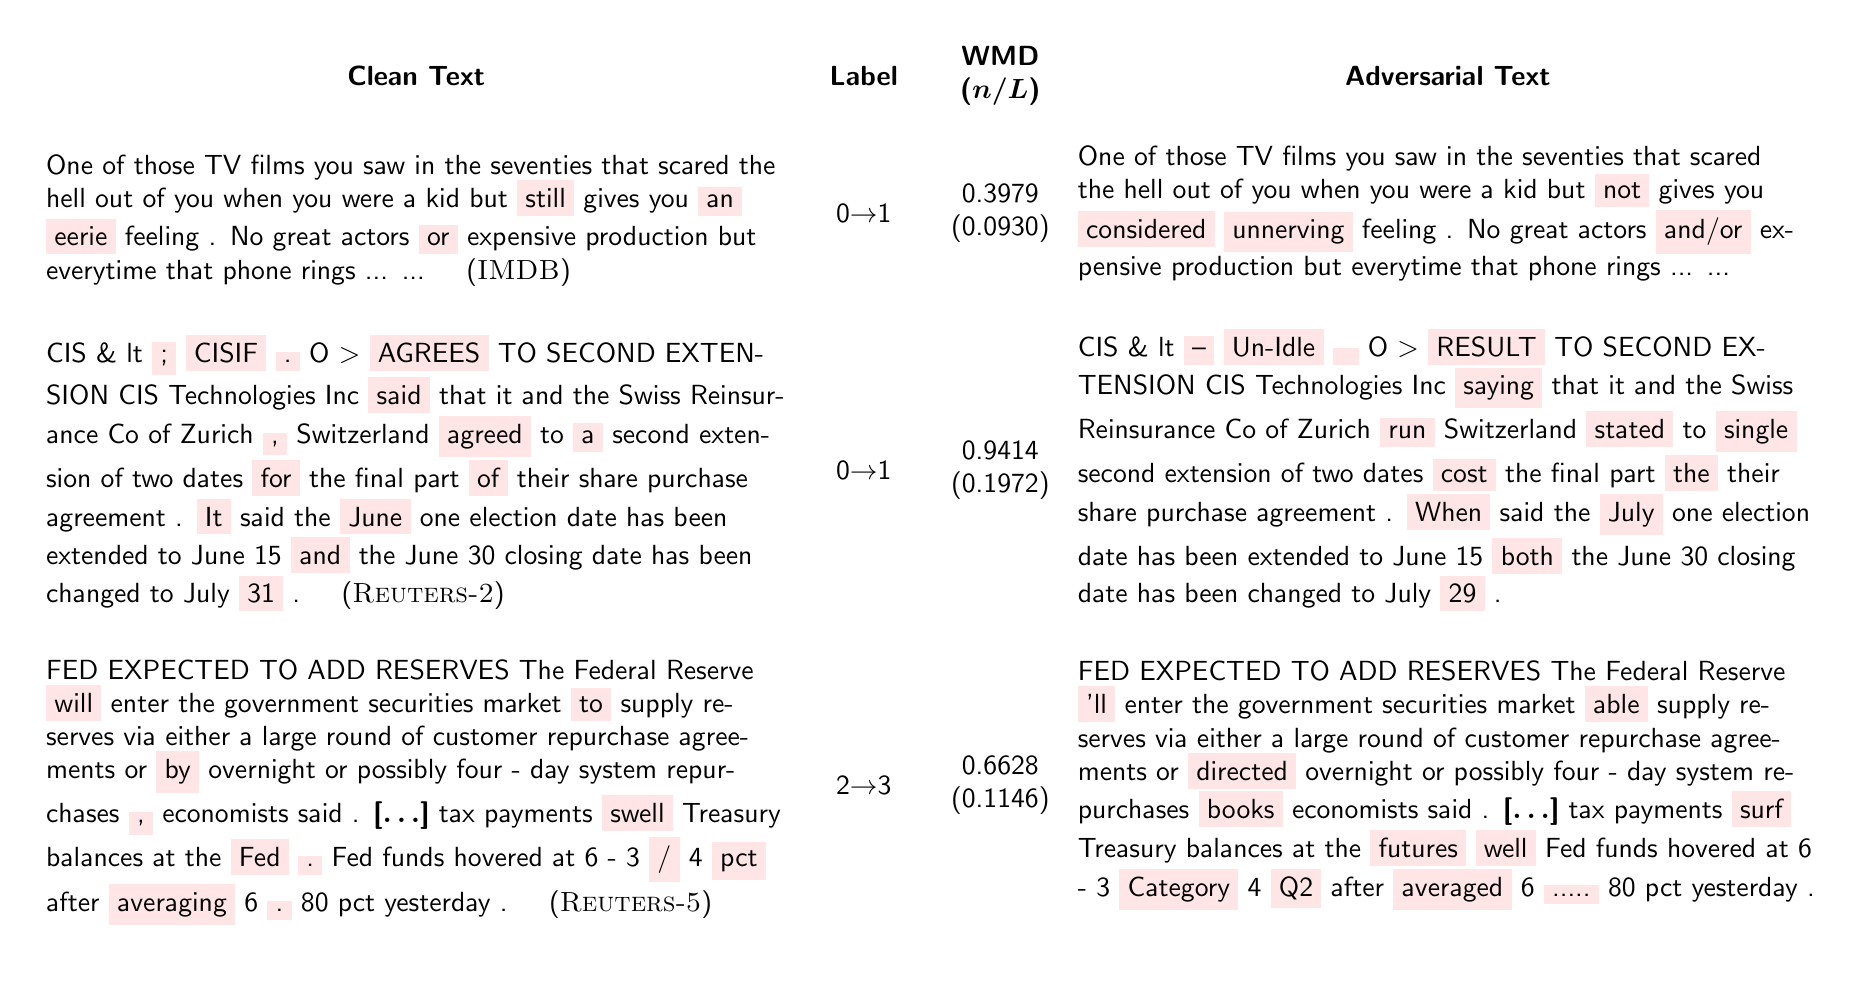
\begin{tikzpicture}
 \matrix[matrix of nodes,every nodes/.style={rectangle},
 row 1/.style={nodes={anchor=center,align=center,font=\bf}},
 row 2/.style={nodes={anchor=north,minimum height=2.5cm}},
 row 3/.style={nodes={anchor=north,minimum height=4cm}},
 row 4/.style={nodes={anchor=north,minimum height=4cm}},
 column 1/.style={nodes={text width=9.4cm}},
 column 2/.style={nodes={text centered, text width=1.5cm}},
 column 3/.style={nodes={text centered, text width=1.5cm}},
 column 4/.style={nodes={text width=9.4cm}}] {
   {Clean Text} & {Label} & {WMD\\(\(\boldsymbol{n/L}\))} & {Adversarial Text} \\

   {One of those TV films you saw in the seventies that scared the hell out of
     you when you were a kid but \hl{still} gives you \hl{an} \hl{eerie} feeling
     . No great actors \hl{or} expensive production but everytime that phone
     rings ... ... \data{IMDB}}

   & {0\(\to\)1}
   & {0.3979\\(0.0930)}

   & {One of those TV films you saw in the seventies that scared the hell out of
     you when you were a kid but \hl{not} gives you \hl{considered}
     \hl{unnerving} feeling . No great actors \hl{and/or} expensive production
     but everytime that
     phone rings ... ...}\\

   {CIS \& lt \hl{;} \hl{CISIF} \hl{.} O \(>\) \hl{AGREES} TO SECOND EXTENSION
     CIS Technologies Inc \hl{said} that it and the Swiss Reinsurance Co of
     Zurich \hl{,} Switzerland \hl{agreed} to \hl{a} second extension of two
     dates \hl{for} the final part \hl{of} their share purchase agreement .
     \hl{It} said the \hl{June} one election date has been extended to June 15
     \hl{and} the June 30 closing date has been changed to July \hl{31}
     . \data{Reuters-2}}

   & {0\(\to\)1}
   & {0.9414\\(0.1972)}

   & {CIS \& lt \hl{--} \hl{Un-Idle} \hl{ } O \(>\) \hl{RESULT} TO SECOND
     EXTENSION CIS Technologies Inc \hl{saying} that it and the Swiss
     Reinsurance Co of Zurich \hl{run} Switzerland \hl{stated} to \hl{single}
     second extension of two dates \hl{cost} the final part \hl{the} their share
     purchase agreement . \hl{When} said the \hl{July} one election date has
     been extended to June 15 \hl{both} the June 30 closing date has been
     changed to July
     \hl{29} .}\\

   {FED EXPECTED TO ADD RESERVES The Federal Reserve \hl{will} enter the
     government securities market \hl{to} supply reserves via either a large
     round of customer repurchase agreements or \hl{by} overnight or possibly
     four - day system repurchases \hl{,} economists said . \ellipsis{} tax
     payments \hl{swell} Treasury balances at the \hl{Fed} \hl{.} Fed funds
     hovered at 6 - 3 \hl{/} 4 \hl{pct} after \hl{averaging} 6 \hl{.} 80 pct
     yesterday . \data{Reuters-5}}
   & {2\(\to\)3}
   & {0.6628 (0.1146)}
   & {FED EXPECTED TO ADD RESERVES The Federal Reserve \hl{'ll} enter the
     government securities market \hl{able} supply reserves via either a large
     round of customer repurchase agreements or \hl{directed} overnight or
     possibly four - day system repurchases \hl{books} economists said
     . \ellipsis{} tax payments \hl{surf} Treasury balances at the \hl{futures}
     \hl{well} Fed funds hovered at 6 - 3 \hl{Category} 4 \hl{Q2} after
     \hl{averaged} 6 \hl{.....} 80 pct yesterday .}\\
 };

\end{tikzpicture}
\end{document}